\documentclass{article}
\usepackage[spanish]{babel}
\usepackage[letterpaper,top=2cm,bottom=2cm,left=3cm,right=3cm,marginparwidth=1.75cm]{geometry}
\usepackage{amsmath}
\usepackage{graphicx}
\usepackage{float} 
\usepackage{pdfpages}
\usepackage[utf8]{inputenc}
\usepackage{biblatex}  
\addbibresource{sample.bib}
\usepackage[colorlinks=true, allcolors=blue]{hyperref}

\title{Reporte Pruebas Piezopulse en Casa del Deporte 08/06}
\author{Isabel Fuentes \\ Vicente Montesinos}
\DeclareUnicodeCharacter{2212}{-}
\begin{document}
\maketitle


\tableofcontents
\newpage
\section{Contextualización}
Piezopulse es una tecnología innovadora diseñada para \textbf{transformar las vibraciones mecánicas generadas por maquinaria industrial en energía eléctrica almacenable}, con el objetivo de reutilizarla dentro del mismo entorno productivo. Este enfoque permite a las empresas mejorar su \textbf{eficiencia energética, reducir costos operativos y alinearse con políticas de sostenibilidad, disminuyendo el desperdicio energético inherente a sus procesos.}\\
\\
Actualmente, el desarrollo se encuentra en una \textbf{fase de evaluación de sistemas de captación y optimización estructural del sistema}, con el objetivo de maximizar la eficiencia de conversión y definir una configuración física  y eléctrica óptima del sistema.
\\
\\
En una \textbf{primera instancia}, se realizaron pruebas en Schussler S.A\cite{PrimeraPrueba}, utilizando como objeto de estudio una \textbf{impresora flexográfica}. La cual forma parte del equipo operativo de la empresa y destaca por encontrarse en constante funcionamiento. Estas pruebas permitieron caracterizar las vibraciones del equipo y \textbf{correlacionarlas con la energía eléctrica} recuperable mediante el sistema. 
\\
\\
Como parte de la \textbf{expansión de escenarios de prueba}, se llevó a cabo una medición en un entorno no industrial: un \textbf{evento deportivo} de alta concurrencia realizado en la Casa del Deporte de la Universidad de Concepción, durante un partido de básquetbol con asistencia masiva de público. Esta instancia permitió explorar el comportamiento del sistema frente a \textbf{vibraciones de baja frecuencia e intensidad variable}, producidas tanto por el movimiento del público como por la presión acústica del ambiente.
\\
\\
El sistema fue ubicado sobre una galería habilitada para los espectadores, con cuatro elementos piezoeléctricos adheridos en su cara inferior, en contacto directo con la estructura. Se evaluaron dos configuraciones eléctricas \textit{(paralelo y serie)} con el objetivo de comparar el voltaje generado bajo cada disposición. Estas pruebas permiten enriquecer la caracterización del sistema en contextos dinámicos y no controlados, aportando datos valiosos para \textbf{futuras aplicaciones en entornos industriales complejos o con fuentes de vibración irregulares.}

\begin{figure}[H]
    \centering
    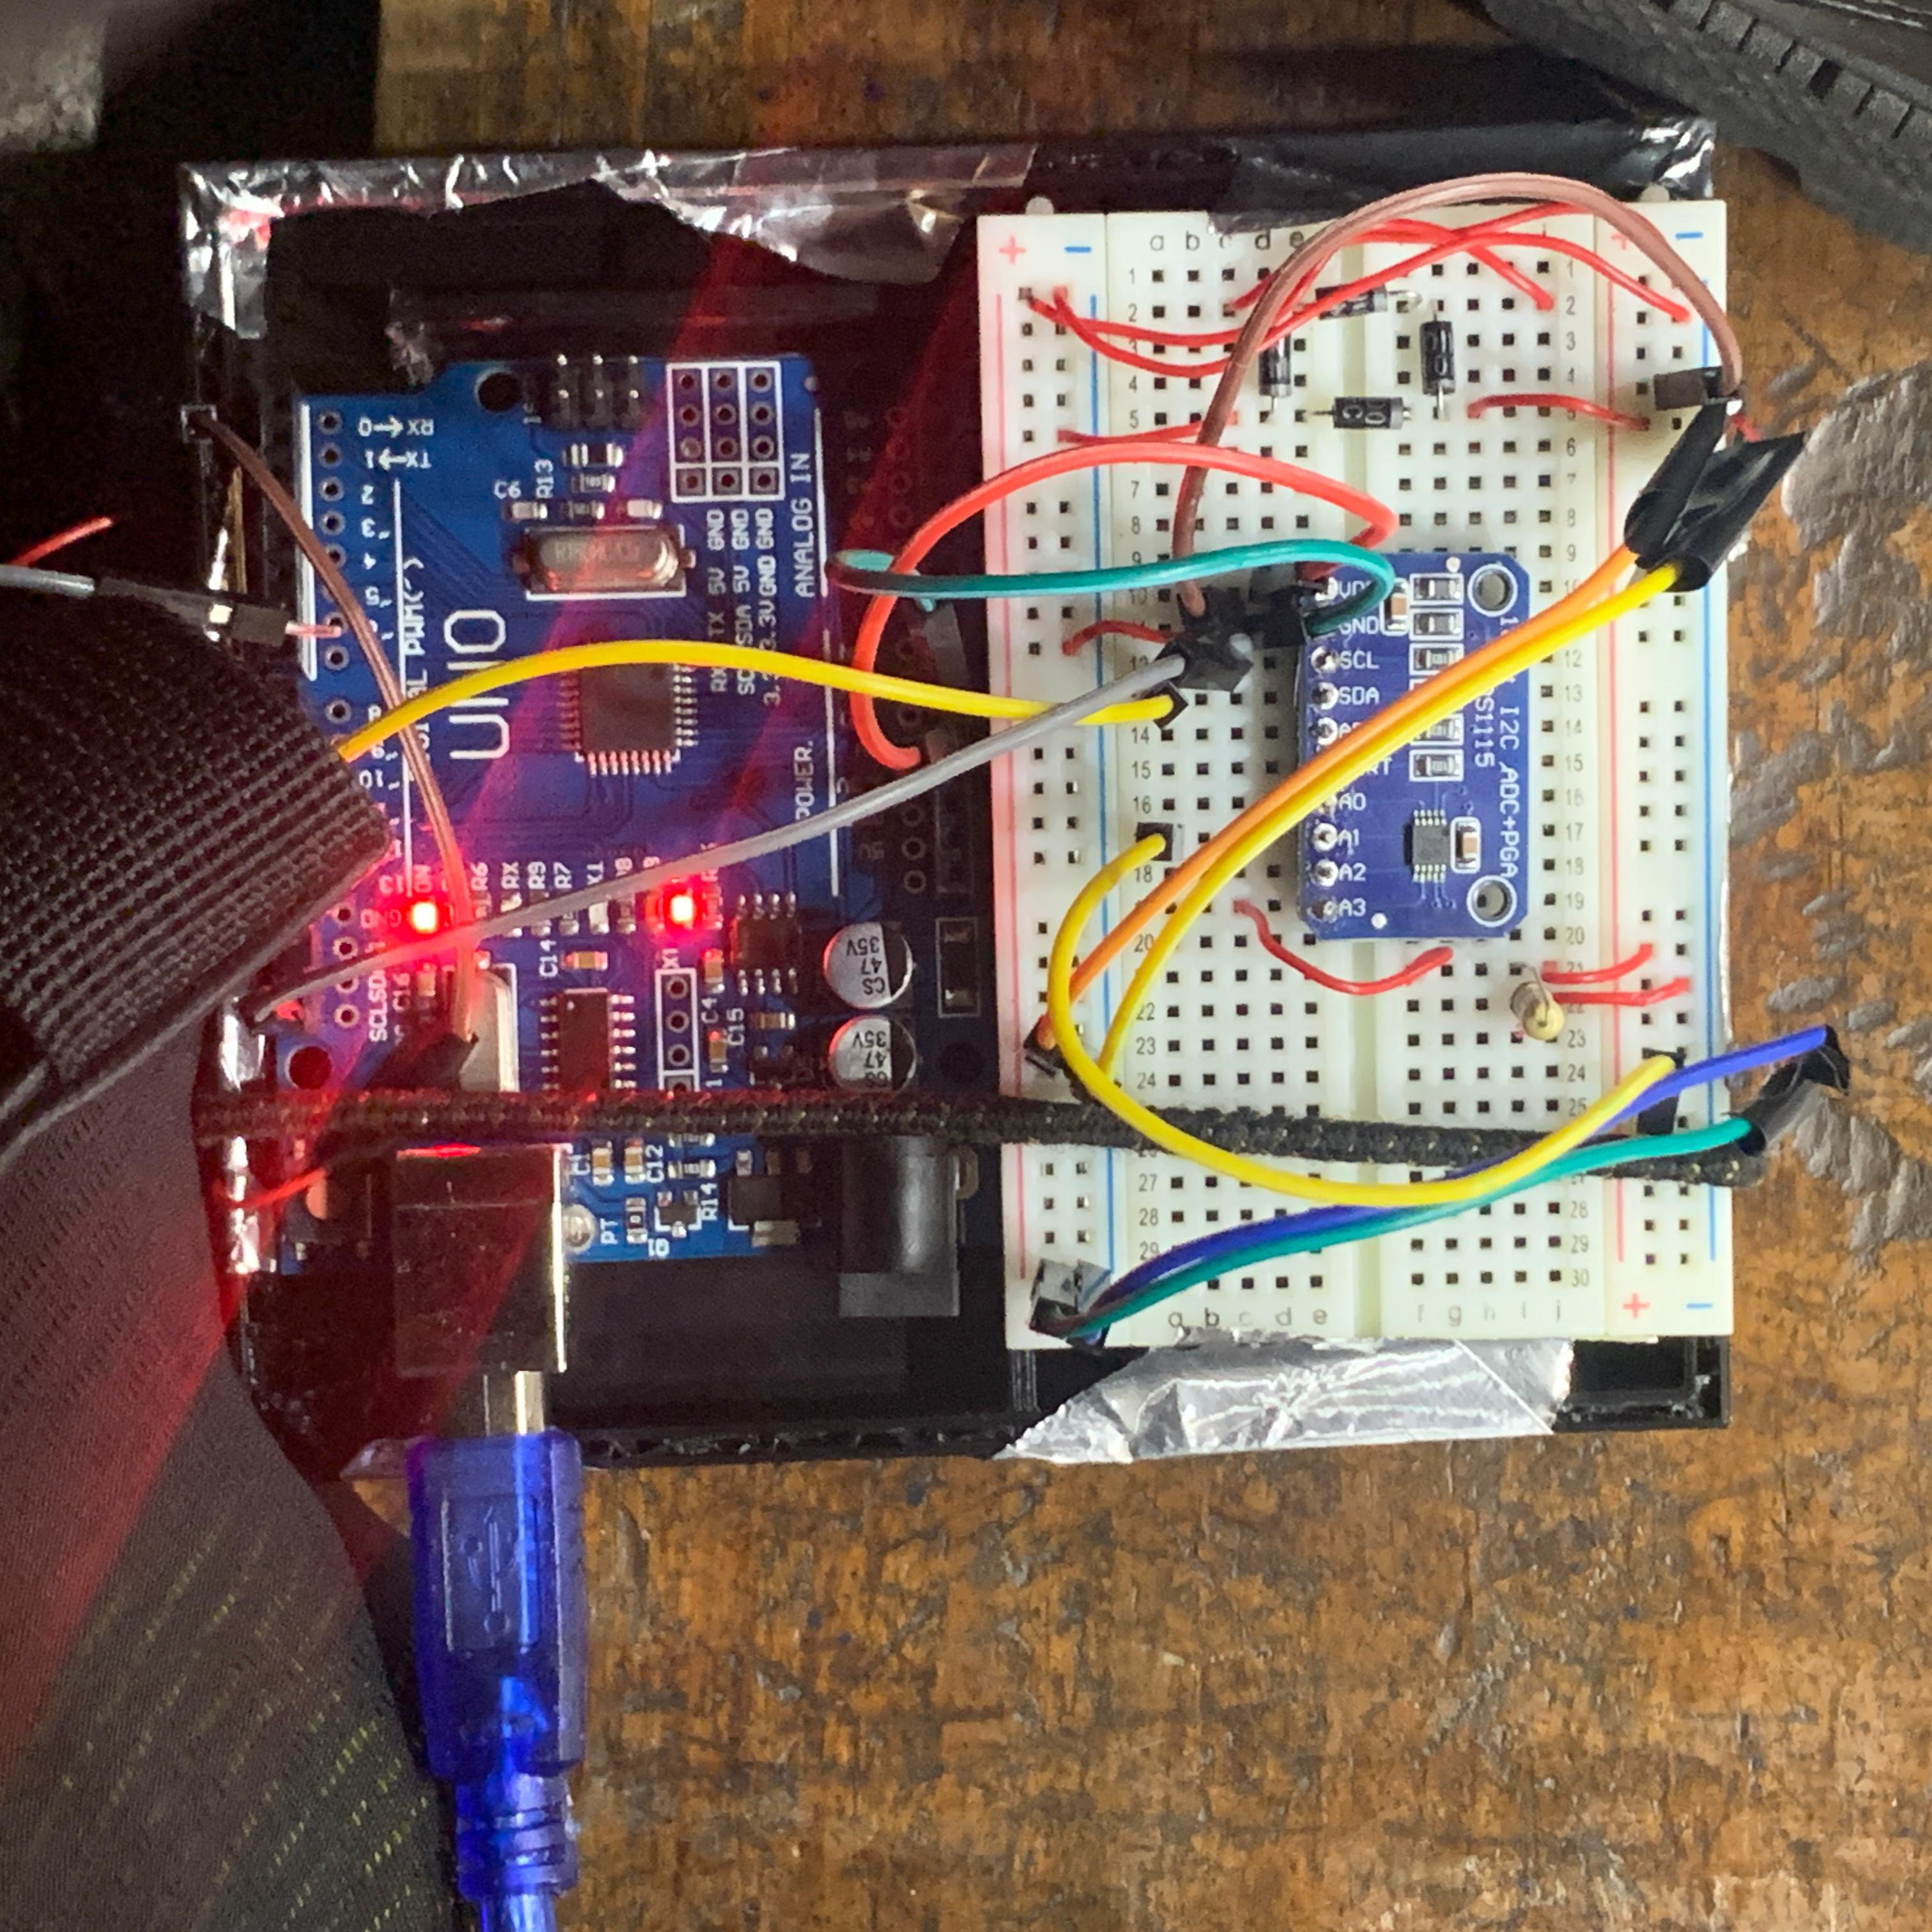
\includegraphics[width=0.5\linewidth]{piezopulse basquetbol.jpeg}
    \caption{Sistema en el sitio de pruebas}
    \label{fig:enter-label}
\end{figure}
\newpage


\section{Configuración Experimental}

El prototipo desarrollado para las pruebas realizadas durante el partido de básquetbol incorporó los siguientes componentes clave, organizados de la siguiente manera:

\subsection{Captación de energía}

El sistema de captación de energía está compuesto por elementos piezoeléctricos de 35 mm de diámetro. Inicialmente, se utilizaron dos de estos piezoeléctricos, probando dos configuraciones distintas: en \textbf{paralelo}, para \textbf{maximizar la corriente de salida}, y en \textbf{serie}, con el objetivo de \textbf{aumentar el voltaje generado}.
\begin{figure}[h]
    \centering
    \begin{minipage}{0.48\textwidth}
        \centering
        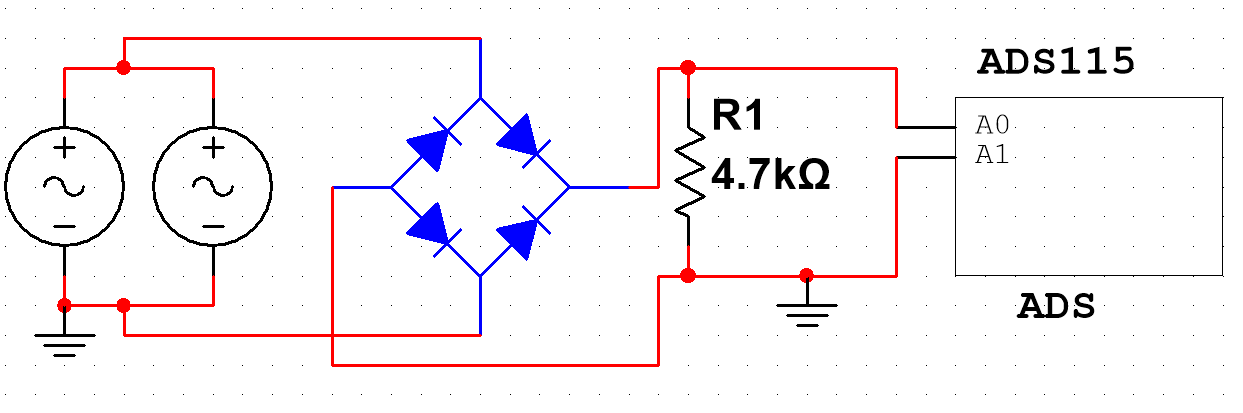
\includegraphics[width=\linewidth]{paralelo.png}
        \caption{Piezoeléctricos en paralelo}
        \label{fig:imagen1}
    \end{minipage}
    \hfill
    \begin{minipage}{0.48\textwidth}
        \centering
        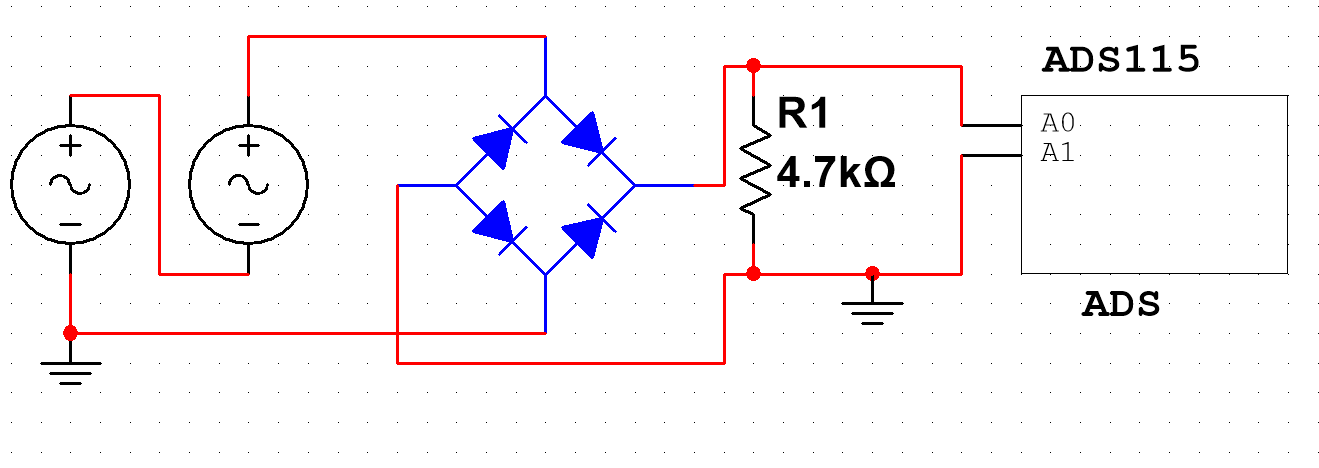
\includegraphics[width=\linewidth]{serie.png}
        \caption{Piezoeléctricos en serie}
        \label{fig:imagen2}
    \end{minipage}
\end{figure}

Para asegurar una correcta transferencia de las vibraciones hacia los piezoeléctricos, se reutilizó el modelo 3D previamente diseñado para las pruebas en Schussler, el cual, gracias a sus caras de espesor mínimo, facilita la transmisión eficiente de vibraciones\cite{PrimeraPrueba}.\\
\\
Adicionalmente, se diseñó una segunda estructura 3D para alojar la protoboard y el microcontrolador Arduino, lo que simplificó el transporte y brindó mayor estabilidad a las conexiones electrónicas. Ambos módulos fueron unidos mediante cinta metálica tipo foil tape, lo que permitió optimizar el espacio y reducir el riesgo de desprendimiento durante las pruebas. 

\begin{figure}[H]
    \centering
    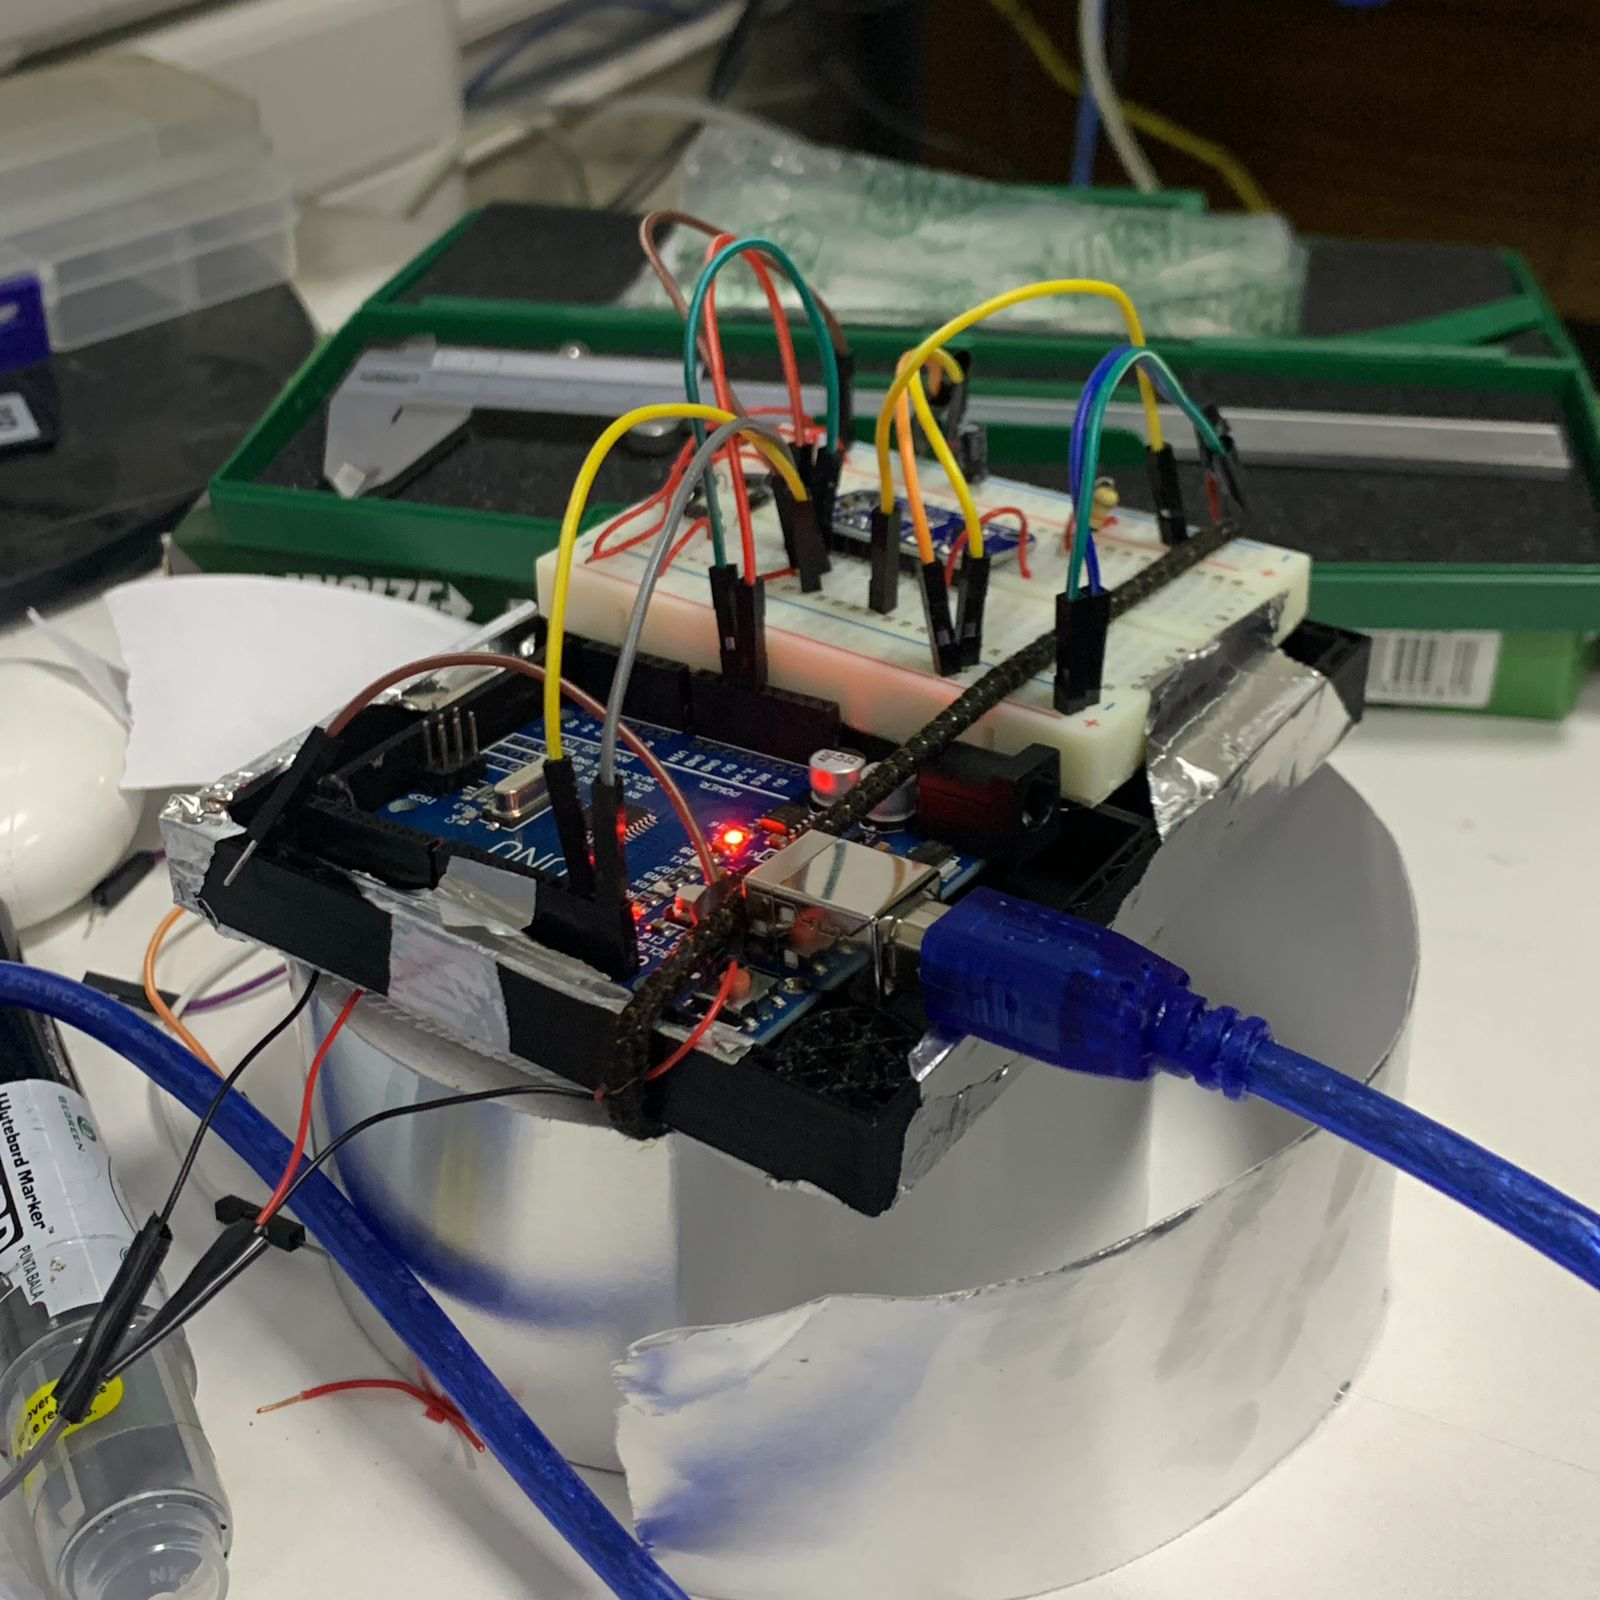
\includegraphics[width=0.5\linewidth]{sistema basquetbol.jpeg}
    \caption{Estructura del sistema electrónico}
    \label{fig:enter-label}
\end{figure}


\subsection{Medición y Adquisición de datos}
El sistema incorpora un conversor analógico-digital ADS1115 configurado en modo diferencial. La entrada positiva A0 se conectó al extremo positivo de una resistencia de 4.97 k$\Omega$, mientras que la entrada negativa A1 se conectó al extremo negativo de la misma resistencia. Esta configuración permitió medir la caída de voltaje directamente a través de la resistencia, aprovechando la alta resolución de 16 bits del ADS1115 para obtener lecturas precisas. El procesamiento y almacenamiento de los datos adquiridos desde el ADS1115 fueron gestionados por un microcontrolador Arduino Uno que centralizó el funcionamiento del sistema de medición. \cite{CodigoArduino}

\section{Resultados y Análisis}
\subsection{Energía piezoeléctrica}
Durante el partido de básquetbol, se registró el voltaje generado por dos piezoeléctricos conectados en paralelo, los cuales fueron ubicados sobre una grada destinada al público. La señal generada fue medida a través de una resistencia de 4.97k$\Omega$, permitiendo estimar la corriente inducida por las vibraciones del entorno.

\begin{table}[H]
\centering
\begin{tabular}{lccc}
\textbf{ } & \textbf{Mínimo} & \textbf{Máximo} & \textbf{Media} \\
\textbf{Voltaje (mV)} & 32.3 & 47.3 & 41.2 \\
\textbf{Corriente ($\mu$A)} & 6.50 & 9.52 & 8.29 \\
\end{tabular}
\caption{Resumen estadístico del voltaje y corriente con piezoeléctricos ubicados en paralelo.}
\label{tab:resumen_voltaje}
\end{table}

Si bien los niveles de voltaje y corriente obtenidos con solo dos piezoeléctricos son bajos y no permiten, por sí solos, alimentar dispositivos electrónicos de forma directa, los resultados confirman que \textbf{es posible extraer energía a partir de vibraciones en este tipo de entornos}. La consistencia de los valores registrados —sin grandes variaciones pese a la naturaleza dinámica del ambiente— sugiere que el sistema es estable y repetible. Esto refuerza la viabilidad de escalar el sistema: al aumentar la cantidad de piezoeléctricos , optimizar el almacenamiento y acondicionamiento de la señal se podría lograr una captación de energía significativa y útil en aplicaciones reales dentro de espacios con actividad constante, como instalaciones deportivas.\\

Después de un tiempo utilizando el sistema con los piezoeléctricos conectados en paralelo, se modificó su configuración para conectarlos en serie, manteniéndose las mismas condiciones de medición mediante una resistencia de 4.97k$\Omega$.

\begin{table}[H]
\centering
\begin{tabular}{lcccc}
\textbf{ } & \textbf{Mínimo} & \textbf{Máximo} & \textbf{Media} \\
\textbf{Voltaje (mV)} & 0.2 & 12.2 & 3.40\\
\textbf{Corriente ($\mu$A)} & 0.04 & 2.46 & 0.68\\
\end{tabular}
\caption{Resumen estadístico del voltaje y corriente con piezoeléctricos ubicados en serie.}
\label{tab:resumen_voltaje}
\end{table}

Al igual que en la configuración paralela, los resultados muestran que los \textbf{piezoeléctricos continúan generando señal eléctrica ante las perturbaciones del entorno}, a pesar de los bajos niveles de voltaje y corriente. La variación observada en los valores es acotada, lo cual indica una respuesta estable del sistema frente a esta nueva disposición.\\
\\

De los resultados obtenidos se deduce que, contrario a lo que indica la teoría básica (donde una conexión en serie debería aumentar el voltaje total) en la práctica esto no se reflejó debido a que \textbf{las señales generadas por los piezoeléctricos tienden a cancelarse entre sí cuando están en serie}. Por otro lado, la configuración en paralelo no presenta esta limitación, lo que representa una ventaja significativa, ya que además del voltaje estable, se observa un \textbf{aumento en la corriente total generada}.
\\
Aún utilizando una cantidad reducida de piezoeléctricos y bajo condiciones estructurales no optimizadas para la transmisión de vibraciones, es posible generar energía eléctrica aprovechable a partir de las vibraciones en ambientes como gradas deportivas. \textbf{Con un diseño escalable este tipo de tecnología podría ser implementada para alimentar dispositivos o sistemas auxiliares en espacios deportivos y otros entornos con actividad constante y vibraciones repetitivas}.\\
Considerando los voltajes de ambas disposiciones durante el muestreo se obtienen los siguientes gráficos:
\begin{figure}[H]
    \centering
    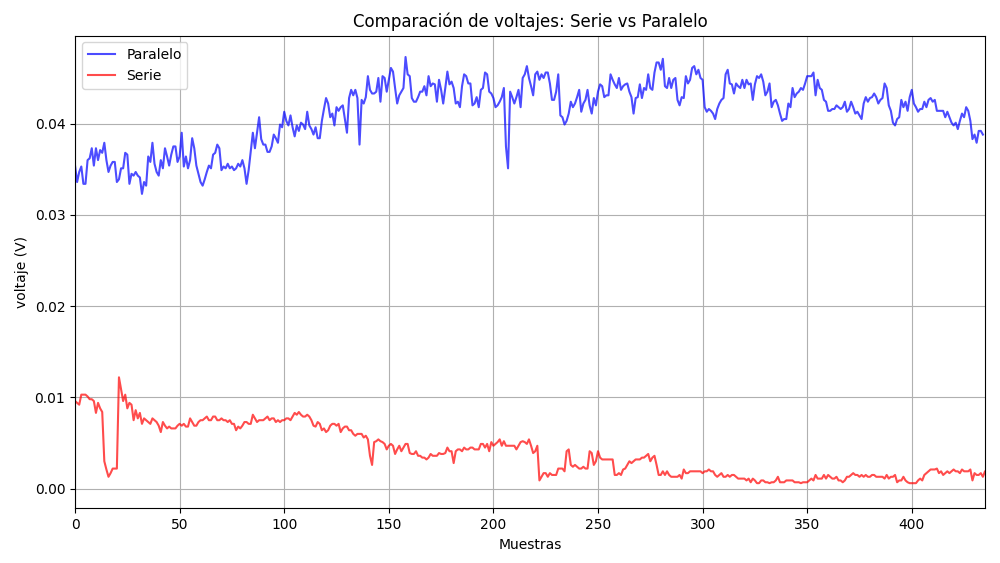
\includegraphics[width=0.9\linewidth]{voltajes.png}
    \caption{Voltajes obtenidos para ambas disposiciones durante el muestreo. }
    \label{fig:enter-label}
\end{figure}
\section{Aplicación del sistema y enfoque sostenible}
Posterior al análisis realizado a las mediciones obtenidas y la consideración de las características del medio en que fué realizado el testeo, \textbf{la tecnología presentada presenta las condiciones aptas para exponerse en entornos sociales donde la participación de los espectadores corresponde a la fuente de vibraciones mecánicas captadas}. Considerando posteriores optimizaciones del sistema para mayor recepción y un mantenimiento de la estructura posibilitando su transporte y ubicación, el carácter de \textbf{sostenible} se hace presente de forma relevante dentro de la descripción de la tecnología.\\
En la actualidad, la implementación de tecnologías que permiten limitar o cesar el uso de fuentes de energías no renovables o estándares y que, cumplen con cualidades como sustentabilidad y sostenibilidad, presentan gran relevancia y consideración en su implementación. La sostenibilidad por su parte, se describe como la capacidad de satisfacer las necesidades del presente sin comprometer la capacidad de las generaciones futuras para satisfacer sus propias necesidades; considerando las repercusiones sociales, medioambientales y económicas de las decisiones que se toman en la actualidad. Ante la problemática del uso de fuentes típicas de energía y sus consecuencias sociales, ambientales y productivas, proponer desarrollos tecnológicos que entreguen soluciones adecuadas a los requerimientos mencionados se presenta como importante. \\
\\
La tecnología Piezopulse cumple con el carácter de \textbf{sostenible}, no modificando el ambiente en el que se aplica y aprovechando las condiciones de este mismo sin generar consecuencias. Es de esta forma que se presenta con grandes ventajas ante otros desarrollos tecnológicos similes, \textbf{destacando por su fácil incorporación en los sitios u objetos que experimentan vibraciones sin alterar su funcionamiento y ocupando un espacio limitado en la estructura}. Es de esta forma que Piezopulse en sus etapas incipientes se presenta con un potencial excepcional como \textbf{fuente de energía verde}, proyéctandose de forma alentadora para su aplicación en desarrollos posteriores mejorados y su futura implementación en el ambiente como fuente de energía verde.









\section{Conclusión y próximos pasos}
Las pruebas realizadas durante el partido de básquetbol en la casa del deporte UdeC permitieron validar el objetivo de funcionamiento y diseño de Piezopulse: \textbf{transformar vibraciones presentes en entornos reales en energía eléctrica utilizable mediante piezoeléctricos}. Como segundo testeo realizado en entorno real, se puede destacar:
\begin{itemize}
    \item Validación de la tecnología en entorno fuera del industrial, permitiendo ampliar su aplicación futura como solución tecnológica a espacios cotidianos donde existen vibraciones mecánicas.
    \item Una distribución en paralelo de los piezoeléctricos permite rescatar más energia. Esto ocurre, debido a que, los piezoeléctricos al estar conectados en serie y a un sistema con vibraciones irregulares existe la posibilidad de que se cancelen mutuamente.
\end{itemize}
Como pasos a futuro con el fin de escalar el desarrollo de la tecnología y continuar con su validación en entornos reales, se propone:
\begin{itemize}
    \item Incorporación de más piezoeléctricos dispuestos en ambas conexiones
    \item Integrar un sistema que permita acumular la energía generada 
\end{itemize}
\printbibliography





\end{document}
